\newcommand{\posterNumbers}[1]{

\setlength{\frameWidth}{#1}
\setlength{\unitlength}{0.02\frameWidth}
\psset{unit=\unitlength}


\rput[lb](0,15){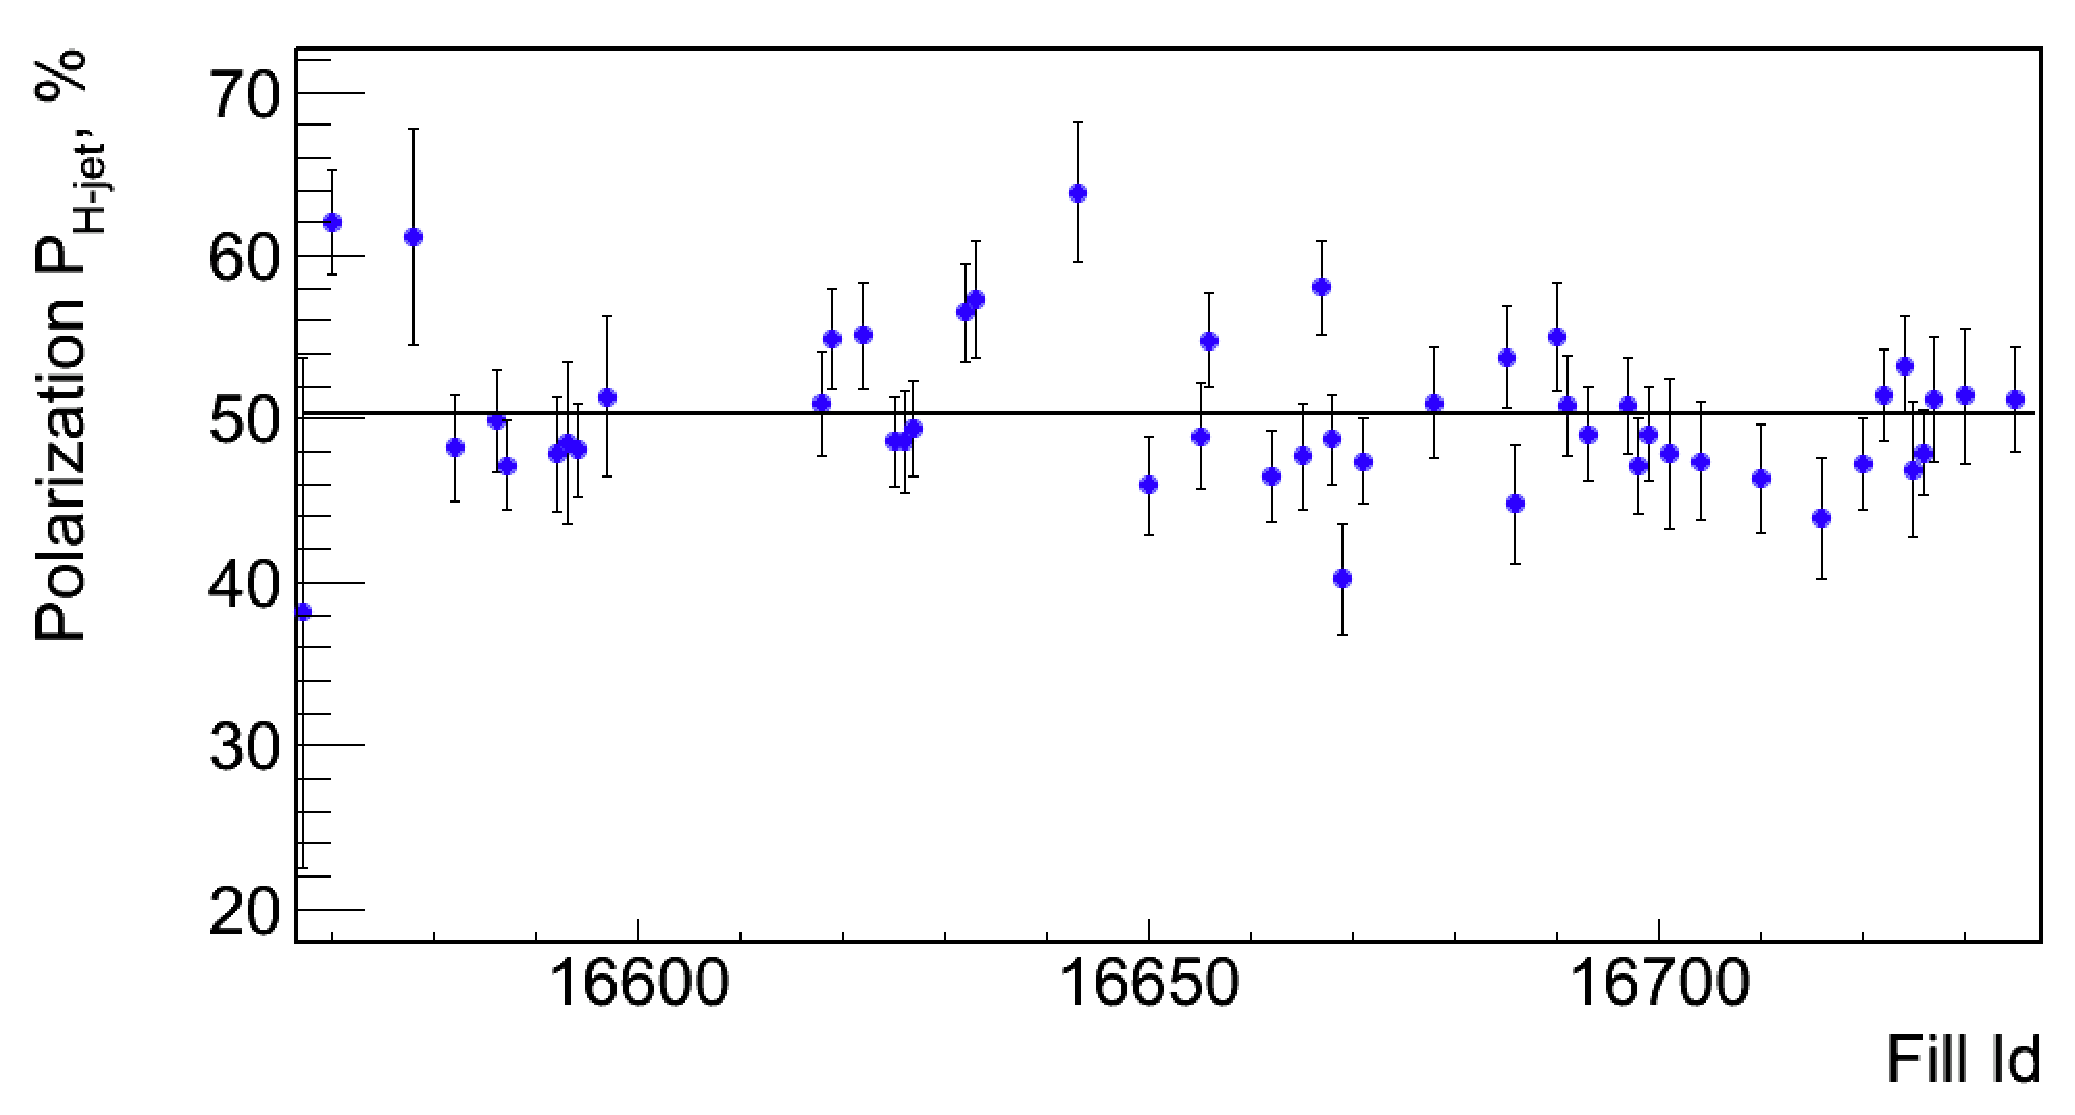
\includegraphics[width=28\unitlength]{graphics/polar_hjet_run12}}
\rput[lt](4,13.5){
\includegraphics[width=24\unitlength]{graphics/target2_0017}}

\rput(16,20){ \psframebox{\small Polarization in Blue ring in 2012 RHIC Run} } 

\rput[lt](30,27) 

	\item In RHIC \textbf{average} beam polarization was {\large $52$~\%} and {\large $58$~\%} for two periods in 2012

	\item Polarization \textbf{losses} are {\large $\frac{dP}{dt} \sim -0.5\%$} per hour during a fill

	\item Relative measurement \textbf{uncertainty} per fill is {\large $\frac{\Delta P}{P} \sim 5\%$}

\end{list}

\end{minipage}
}


%\rput{0}{\psgrid[gridlabels=0.7,subgriddiv=0, griddots=3](1,-1)(0,0)(\myPsPictureWidthLocal,\myPsPictureHeightLocal)}

}

\setlength{\unitlength}{10mm}
\psset{unit=\unitlength}
